\chapter{Real-Time Scheduling}

\section{Introduction}
It has become common for current mobile devices to use asymmetric mobile processors. 
The state-of-the-art leading processor architecture for this purpose is the ARM big.LITTLE architecture that combines fast out-of-order big cores with simple in-order little cores in order to achieve high performance in a low power budget. 
Scheduling of tasks on such architectures becomes more challenging as an efficient scheduler has to take into account the asymmetry of the system in order to maintain load balance. 
The state of the art Linux scheduler named “Completely Fair Scheduler” (CFS) manages to be fair by allowing tasks to execute for the same amount of time on each processor. 
This contradicts to the needs of an asymmetric system as a fair distribution of the tasks on an asymmetric system would lead to load imbalance and wrong scheduling decisions. 
Heterogeneous Multi-Processing (HMP) is an enhancement in CFS towards the solution of this challenge. 
However, our primary investigation on games showed that even by using HMP in CFS, the system is not always taking the right decisions for task migration. 
From our profiling and evaluation of this existing scheduler, we saw that most of the times, critical threads of the game are scheduled on little cores of the system, causing a drop to the FPS, which makes the user less satisfied. 
This was our initial motivation for proceeding in the direction of implementing a scheduling solution that takes into account the importance of some threads as well as the asymmetry of the system.


\begin{figure}[t]%
	\centering
	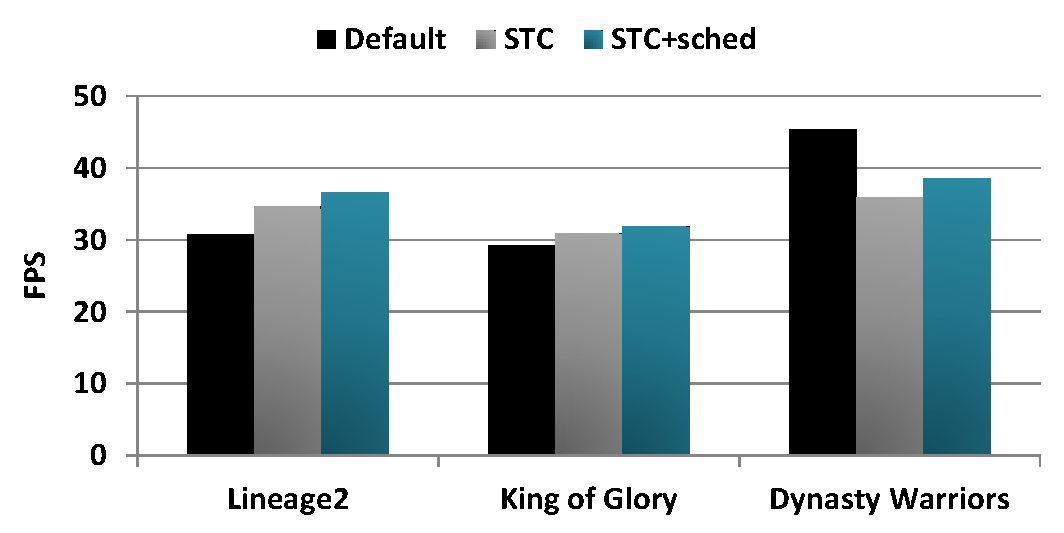
\includegraphics[width=0.7\textwidth]{figures/FPS.pdf}
	\caption{FPS.}
	\label{fig:FPS}
\end{figure}

\begin{figure}[t]%
	\centering
	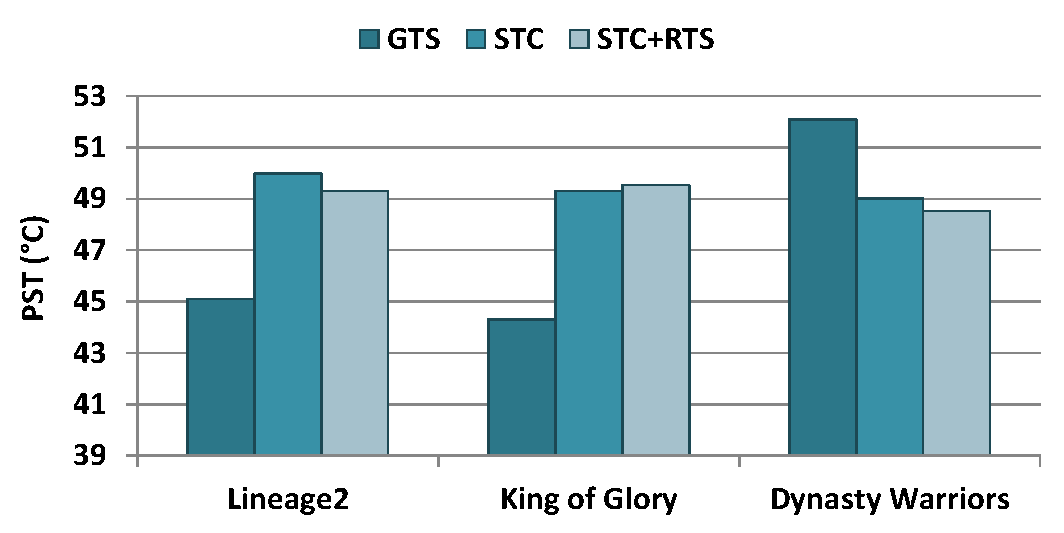
\includegraphics[width=0.7\textwidth]{figures/PST.pdf}
	\caption{PST.}
	\label{fig:PST}
\end{figure}


\begin{figure}[t]%
	\centering
	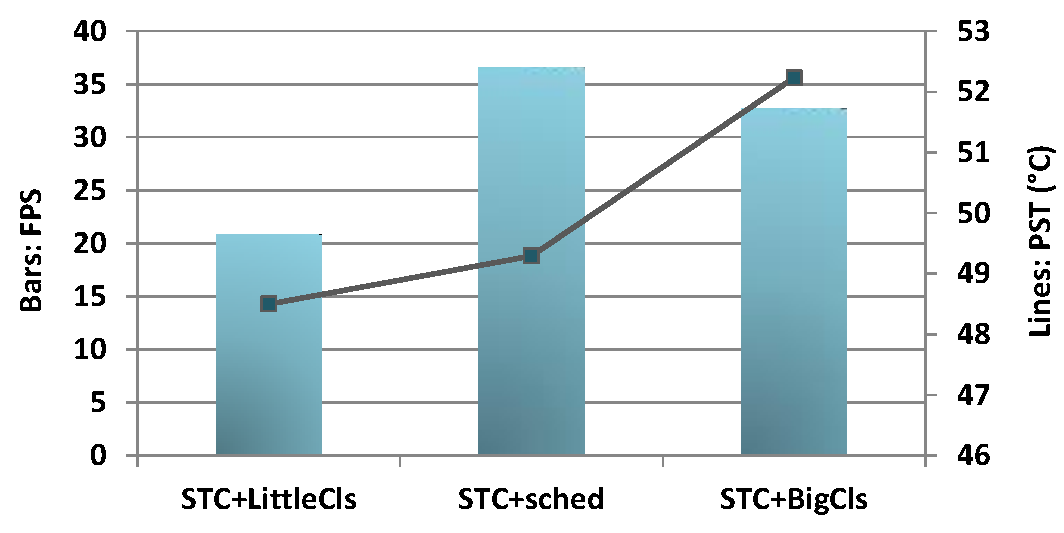
\includegraphics[width=0.7\textwidth]{figures/intern_comparison.pdf}
	\caption{Comparison.}
	\label{fig:int_comparison}
\end{figure}


The goal of this internship was to improve game performance (frames per second, FPS) through scheduling of tasks on mobile devices. To approach this challenge we had to break the problem into several steps. Below we briefly describe the steps taken:
1.	Profiling and evaluation of the baseline: at this step we conducted a study to explore the current performance and limitations of the device while running games. An initial evaluation proved that there is room of improvement of frame rate by modifying the scheduling as well as other parameters of the governor.
2.	Design process: in this step we explored the possibilities of implementing a scheduler. This step was the pathway to the implementation of a final solution as it led us to choose the appropriate programming framework to implement a scheduling solution. This was based on the programming flexibility as well as on the available tools and resources.
3.	Implementation and experimentation: In this step, after the design and software core implementation was done, we experimented with different policies and tuned the scheduler until we reached the desired result.
4.	Evaluation: In this step we evaluated our solution on several different games. We compared our solution against the baseline as well as against other mainstream scheduling solutions that we implemented and we got satisfactory results.

Summary of research results, publications, project proposals produced

During the design process we experimented with different levels of the software stack for finding the most appropriate level for such an implementation. From this study we concluded that scheduling in the kernel level requires a lot of time and is not flexible. An important drawback of the kernel level scheduling is that information provided at this level is limited. For example there is no way to know what each task is used for and what the current runtime circumstances are. This led us to move upwards in the software hierarchy and built up the circumstances to reuse existing Samsung software and implement our solution within a system service that starts execution whenever it detects that a game application is running.
The next step was to find the appropriate scheduling policy. This would include the data and runtime circumstances that the scheduler should use to make scheduling decisions. From this step we found that temperature plays a very important role in FPS performance. Thus we used this information to make scheduling decisions for the tasks of the executing game. When our scheduler detects that the temperature increases, it gradually starts migrating tasks of the game to the little cluster. In the opposite scenario, when temperature is decreasing the scheduler manages to migrate tasks that run on the little cluster, back to the big cluster. Finding the correct balance between temperature and task migration required a lot of experimentation and profiling of our solution. 
The final step of our activities was to evaluate our approach. We used three different games: Lineage2, King of Glory and Dynasty Warriors. The specific games were selected because they fulfilled the following criteria:
1.	High FPS up to 60 and demanding graphics
2.	Auto-play mode
3.	Playing with no intervals for a long time
We conducted experiments using our policy on top of Samsung’s Temperature Control (STC) framework used to maintain the temperature to the desired levels. We compare our results to the default version of STC and to the default version without using STC. Our experiments include 10 runs for each game-scheduler pair and each run takes up to 800 seconds. The reported results show the average among the 10 runs.


Figure 1 shows the median FPS obtained from three games using the three different scenarios described above. STC+sched approach improves STC by 6\% for Lineage2, by 3\% for King of Glory and by 7.5\% for Dynasty Warriors. An interesting observation is that for Dynasty Warriors the default approach with no temperature control has no benefit from the approaches that control temperature. This is because in this case the default Linux governor and scheduler constantly push the system to achieve higher FPS increasing the temperature of the device as shown in Figure 2. With this approach, when the temperature increases to a critical point, the device crashes as it has to shut down due to very high temperature.
The FPS stability is another important characteristic of the game execution. This metric characterizes how stable is the FPS during the gameplay. We compute the stability by representing the percentage of FPS readings that are at maximum 20\% above or below the median FPS. Figure 3 shows that FPS stability is not affected by the task scheduling performed by our approach even if tasks migrate to different CPU clusters.

Finally, we compare our scheduler against two different scheduling approaches that do not involve any sophisticated task migration: 
1.	LittleCls: in this approach all the tasks of the game are maintained in the little cluster
2.	BigCls: in this approach all the tasks of the game are maintained in the big cluster
Figure 4 shows the FPS and temperature results for the above scheduling approaches. This figure is used to prove that our solution is effective due to the runtime decisions taken according to the current temperature and runtime circumstances.

